\chapter{Ana's plan}\label{Intro}
I've asked ChatGPT to build me a syllabus:
\begin{enumerate}
    \item \href{https://www.youtube.com/watch?v=fa0zHI6nLUo&list=PLbMVogVj5nJTZJHsH6uLCO00I-ffGyBEm}{Fluid Mechanics}: Conservation of mass, momentum (Navier-Stokes equations), incompressible flows.
    \item Rheology and Non-Newtonian Fluids \begin{Figure}
    \centering
    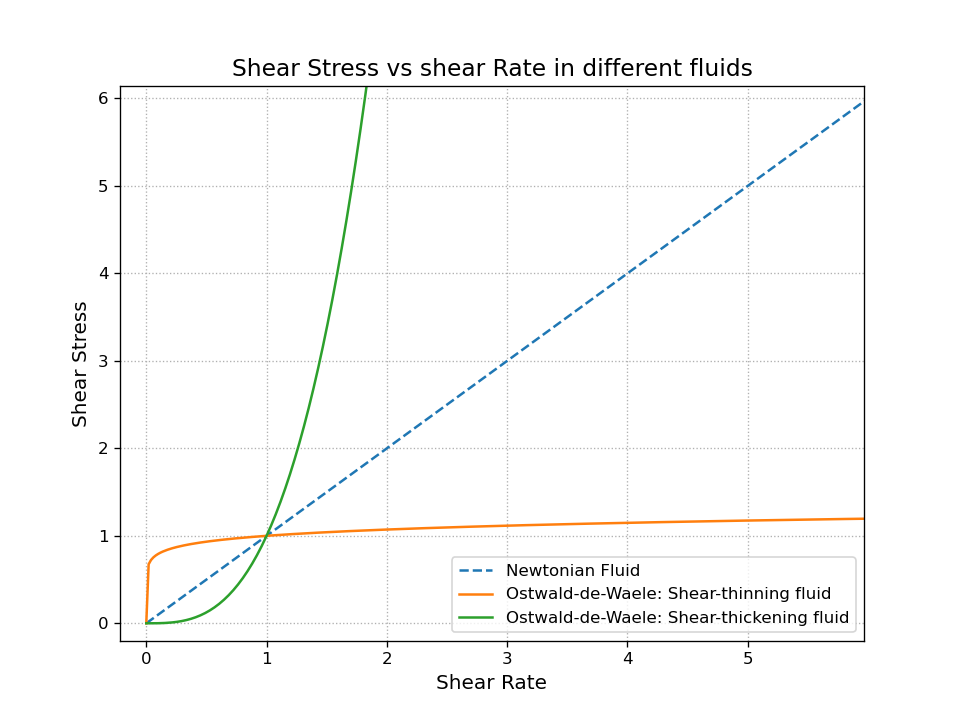
\includegraphics[width=0.9\linewidth]{types_of_fluids.png}
    \captionof{figure}{Newtonian vs. non-Newtonian behaviour, Shear Stress and shear Rate relationships.}
    \label{fig:fluids_types}
    \end{Figure}
    \item Stokes' equations. Methods for solving PDEs, boundary conditions, numerical methods.
    \item Glaciology Key Topics: Ice deformation, creep processes, thermal effects.%Suggested Resources: "The Physics of Glaciers" by W.S.B. Paterson.
    \item Numerical Methods for solving the Stokes equations can help since these equations often don't have analytical solutions.
    % Key Topics: Finite element methods (FEM), finite difference methods (FDM). Suggested Resources: "Numerical Recipes: The Art of Scientific Computing" by Press et al. and "Computational Rheology" by Owens and Phillips.
\end{enumerate}



% \begin{Figure}
% \centering
% 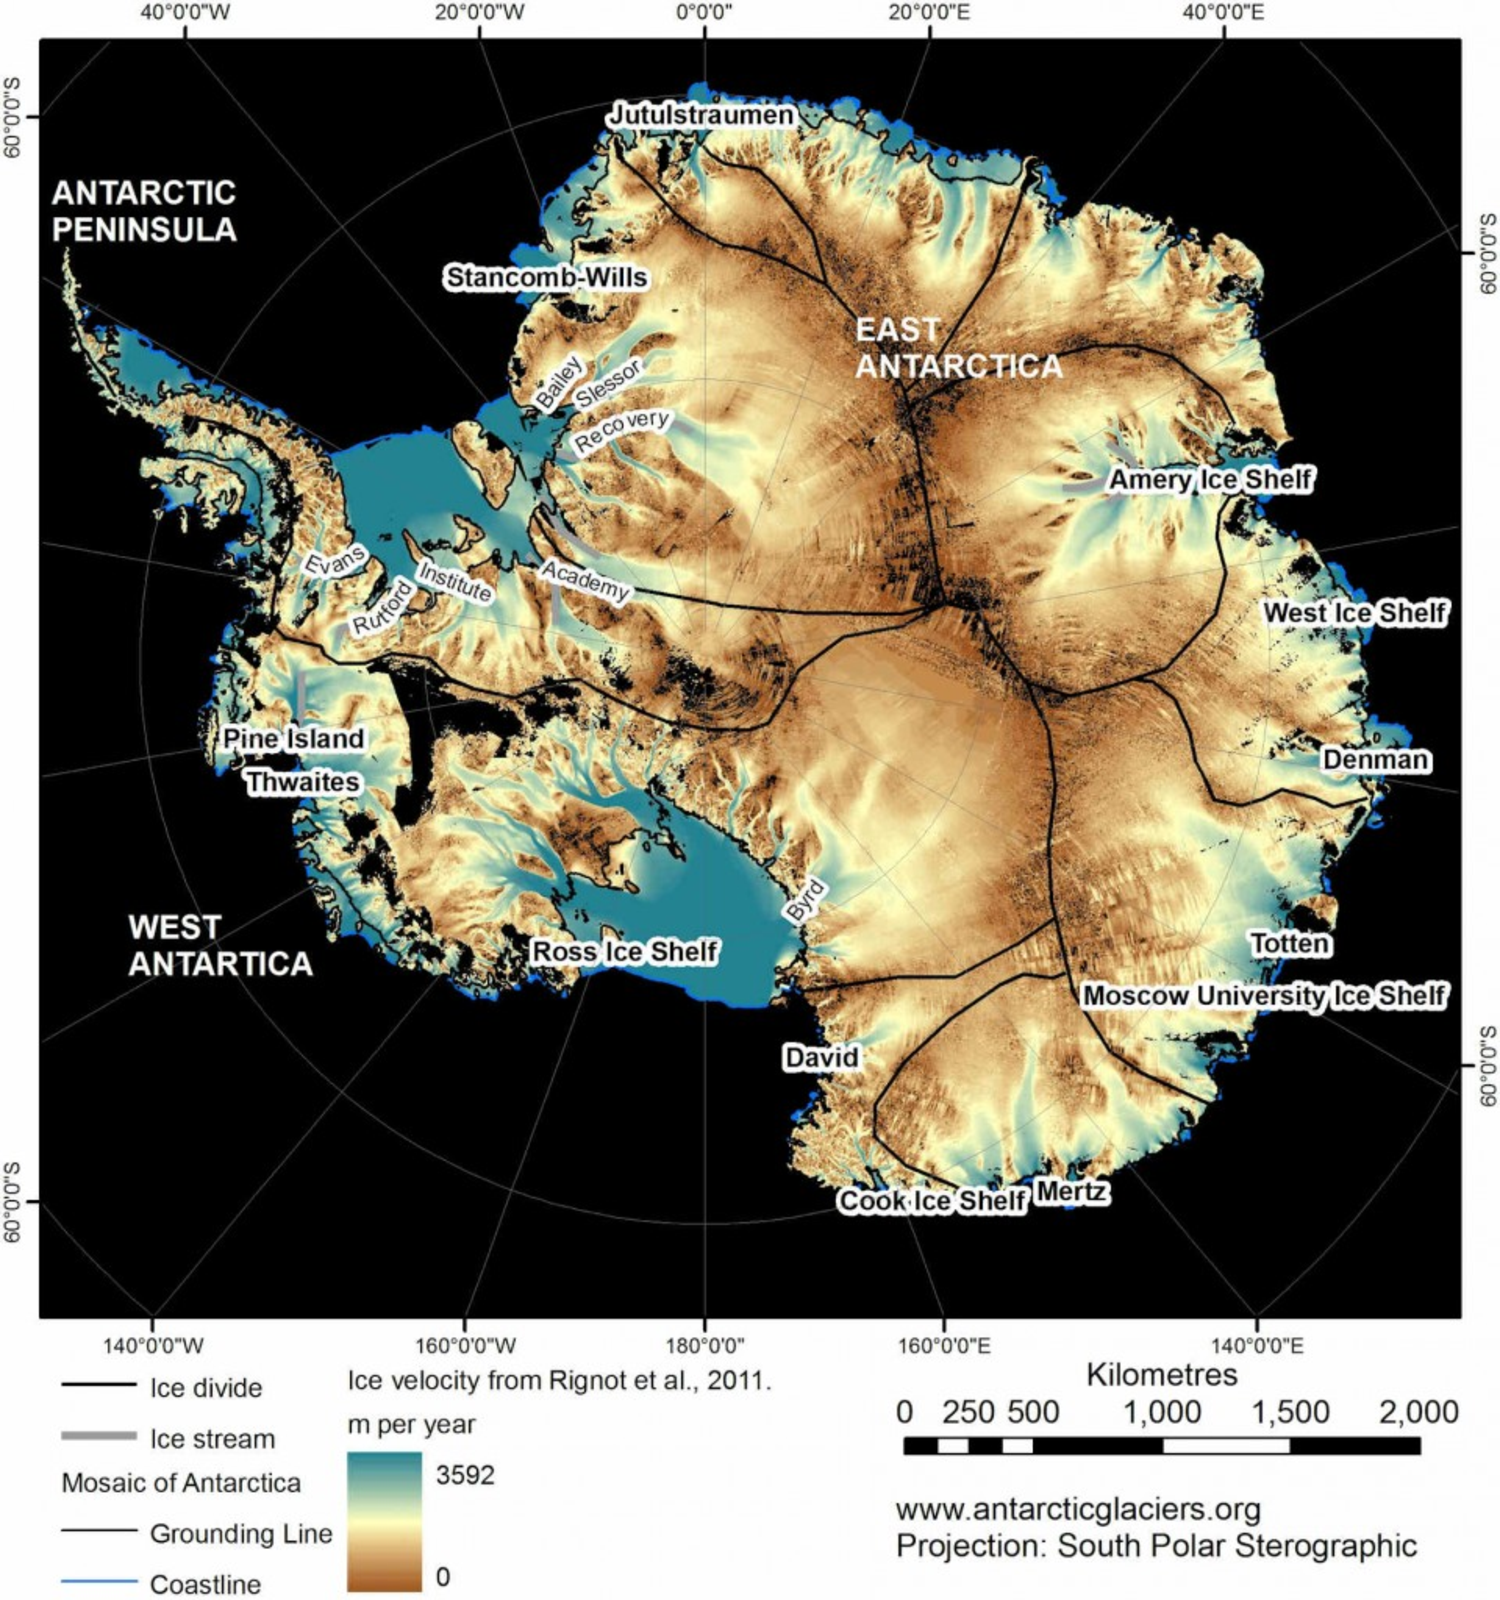
\includegraphics[width=1\linewidth]{antarctica_velocity.pdf}
% \captionof{figure}{}
% \label{fig:Antarctica_velocity}
% \end{Figure}

